\documentclass[a4paper,10pt,twocolumn]{article}

\usepackage[UTF8,fontset=fandol]{ctex}
\usepackage{amsmath,amssymb}
\usepackage{graphicx}
\usepackage{booktabs}
\usepackage{geometry}
\usepackage{hyperref}
\usepackage{caption}
\usepackage{array}
\usepackage{float}
\usepackage{listings}
\usepackage{xcolor}

\geometry{a4paper,margin=1.7cm,columnsep=0.75cm}
\setlength{\parindent}{2em}
\setlength{\parskip}{0.25em}
\renewcommand{\arraystretch}{1.15}

\lstset{
  language=Python,
  basicstyle=\ttfamily\scriptsize,
  keywordstyle=\color{blue!70!black},
  commentstyle=\color{gray!80!black},
  stringstyle=\color{green!40!black},
  numbers=none,
  columns=fullflexible,
  keepspaces=true,
  breaklines=true,
  breakatwhitespace=true,
  frame=single,
  showstringspaces=false,
  xleftmargin=0.4em,
  framexleftmargin=0.4em,
  aboveskip=0.4em,
  belowskip=0.4em
}


\title{课程报告一：手搓多层神经网络}
\author{方俊睿\\学号：3230104069}
\date{}


\begin{document}
\maketitle

\section{问题1：反向传播算法的计算图表示}

我对反向传播的理解是：先把网络前向计算拆成一个个小步骤（也就是计算图里的节点和边），然后再按相反方向把梯度传回来。这样做的好处是每一步都很清楚，哪里算错、哪里梯度变小，都比较容易定位。对多层感知机来说，每层都可以写成
\[
a^{(l-1)} \rightarrow z^{(l)} \rightarrow a^{(l)} \rightarrow \mathcal{L}
\]
也就是“线性变换 $\rightarrow$ 激活函数 $\rightarrow$ 损失函数”这条链路。

\begin{figure}[H]
\centering
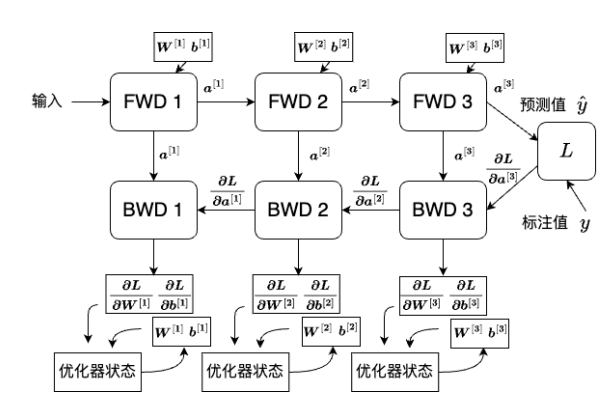
\includegraphics[width=0.95\columnwidth]{计算图.jpg}
\caption{反向传播计算图示意}
\end{figure}

以前馈网络第 $l$ 层为例，前向计算是：
\[
z^{(l)} = W^{(l)}a^{(l-1)} + b^{(l)},\qquad a^{(l)}=f\bigl(z^{(l)}\bigr)
\]
其中 $a^{(0)}=x$，输出层 $a^{(L)}=\hat{y}$。如果第 $l$ 层有 $m^{(l)}$ 个神经元，那么
\[
W^{(l)}\in\mathbb{R}^{m^{(l)}\times m^{(l-1)}},\quad
b^{(l)}\in\mathbb{R}^{m^{(l)}},\quad
a^{(l)}\in\mathbb{R}^{m^{(l)}}
\]
这个维度关系保证了各层矩阵乘法能对上。

反向传播本质上就是链式法则：
\[
\text{标量：}\ \frac{dz}{dx}=\frac{dz}{dg}\frac{dg}{dx},\qquad
\text{向量：}\ \frac{\partial z}{\partial \mathbf{x}}
=\frac{\partial \mathbf{y}}{\partial \mathbf{x}}
\frac{\partial z}{\partial \mathbf{y}}
\]
放到计算图里看，就是每个节点先接收“上游梯度”，再乘当前节点的“局部导数”。

若损失函数为 $\mathcal{L}$，定义误差项
\[
\delta^{(l)} = \frac{\partial \mathcal{L}}{\partial z^{(l)}}
\]
则输出层和隐藏层的反向递推分别为：
\[
\delta^{(L)}=\frac{\partial \mathcal{L}}{\partial a^{(L)}}\odot f'\bigl(z^{(L)}\bigr)
\]
\[
\delta^{(l)}=\left(W^{(l+1)}\right)^T\delta^{(l+1)}\odot f'\bigl(z^{(l)}\bigr)
\]
其中 $\odot$ 为逐元素乘法。

常见激活函数的局部导数：
\[
\sigma'(x)=\sigma(x)\bigl(1-\sigma(x)\bigr),\qquad
\tanh'(x)=1-\tanh^2(x)
\]
\[
\mathrm{ReLU}'(x)=
\begin{cases}
1, & x>0\\
0, & x\le0
\end{cases}
\]
这些导数的大小直接影响梯度会不会变得太小，从而影响训练速度和稳定性。

因此各层参数梯度可统一写为：
\[
\frac{\partial \mathcal{L}}{\partial W^{(l)}} = \delta^{(l)}\left(a^{(l-1)}\right)^T,
\qquad
\frac{\partial \mathcal{L}}{\partial b^{(l)}} = \delta^{(l)}
\]
最后用梯度下降类方法更新参数。整体流程可以概括为：先前向算输出，再算输出层误差，接着逐层反传，最后更新参数。

\section{问题2：基于多层感知机的 FashionMNIST 图像分类实验}

\subsection{问题简介}

这一部分我主要做了一件事：用课程给的 \texttt{demo\_mnist\_ann.py} 自己把 MLP 在 FashionMNIST 上跑通，再看看不同配置到底差在哪。相比只看最终准确率，我更关心的是训练过程本身，比如有没有稳定上升、会不会卡住、不同参数改完后曲线变化大不大。

实验里重点比较了三类因素：激活函数（Sigmoid、Tanh、ReLU、ReLU3）、优化算法（GD、SGD、ADAM）和学习率。评价标准也比较直接：训练集准确率、测试集准确率，以及训练曲线的变化趋势。最后目标是给出一个在当前代码和机器条件下更稳、更好用的组合。

\subsection{模型与算法介绍}

模型用的是最基础的前馈全连接网络。按当前代码，网络结构是
\[
784\rightarrow 128\rightarrow 64\rightarrow 10
\]
输入 784 是把 $28\times 28$ 的图像拉平成向量，输出 10 对应 10 个类别。中间两层隐藏层分别是 128 和 64 个神经元。激活函数支持 Sigmoid、Tanh、ReLU、ReLU3；优化器支持 GD、SGD、ADAM。代码层面还做了 CPU/GPU 双后端，能在 NumPy 和 CuPy 之间切换。

核心计算还是标准的前向 + 反向：
\[
z^{(l)}=W^{(l)}a^{(l-1)}+b^{(l)},\qquad
a^{(l)}=f\!\left(z^{(l)}\right)
\]
\[
\delta^{(l)}=\left(W^{(l+1)}\right)^T\delta^{(l+1)}\odot f'\!\left(z^{(l)}\right)
\]
\[
\frac{\partial \mathcal{L}}{\partial W^{(l)}}=\delta^{(l)}\left(a^{(l-1)}\right)^T
\]
当前实现里损失函数用的是误差平方和（SSE），每个 epoch 按选定优化器更新参数。
需要注意的是，当前实验采用的是误差平方和（SSE）损失，而分类任务中更常见的是交叉熵损失。SSE 在 Sigmoid 输出场景下可能出现梯度偏小的问题，从而影响收敛速度，这也是后续结果分析时需要考虑的因素之一。

三种优化算法可以简单理解为：
\[
\mathrm{GD}:~\theta\leftarrow\theta-\eta\cdot\frac{1}{N}\sum_{i=1}^{N}\nabla_{\theta}\mathcal{L}_i
\]
\[
\mathrm{SGD}:~\theta\leftarrow\theta-\eta\cdot\nabla_{\theta}\mathcal{L}_{i_t}
\]
\[
\mathrm{ADAM}:~
\begin{cases}
m_t=\beta_1 m_{t-1}+(1-\beta_1)g_t\\
v_t=\beta_2 v_{t-1}+(1-\beta_2)g_t^2\\
\theta_t=\theta_{t-1}-\eta\frac{\hat m_t}{\sqrt{\hat v_t}+\epsilon}
\end{cases}
\]
直观上，GD 用全样本平均梯度，SGD 用单样本近似梯度，ADAM 在梯度基础上再做一阶/二阶动量修正，通常调好学习率后更容易得到稳定结果。

\begin{table}[H]
\centering
\small
\caption{模型与训练算法配置}
\begin{tabular}{c|c}
\toprule
项目 & 配置 \\
\midrule
网络结构 & $784\rightarrow 128\rightarrow 64\rightarrow 10$ \\
激活函数 & Sigmoid / Tanh / ReLU / ReLU3 \\
优化算法 & GD / SGD / ADAM \\
损失形式 & 误差平方和（代码实现） \\
计算后端 & NumPy（CPU）/ CuPy（GPU） \\
\bottomrule
\end{tabular}
\end{table}

\subsection{数据集和算例参数介绍}

FashionMNIST 数据集包含 60000 张训练图像和 10000 张测试图像，单张图像大小为 $28\times 28$。为控制计算开销，算例中按不同实验设置抽取部分样本训练与测试。

\begin{table}[H]
\centering
\small
\caption{数据集与算例参数}
\begin{tabular}{c|c}
\toprule
项目 & 数值 \\
\midrule
完整训练集大小 & 60000 \\
完整测试集大小 & 10000 \\
图像尺寸 & $28\times 28$ \\
分类类别数 & 10 \\
典型训练轮次 & 10000 \\
\bottomrule
\end{tabular}
\end{table}

\subsection{结果罗列与汇总}

\textbf{(1) 不同激活函数 + SGD（学习率 0.1）}

\begin{table}[H]
\centering
\scriptsize
\caption{不同激活函数在 SGD 下的结果}
\resizebox{\columnwidth}{!}{
\begin{tabular}{ccccccc}
\toprule
训练轮次 & 激活函数 & 学习率 & 训练样本数 & 测试样本数 & 训练集准确率 & 测试集准确率 \\
\midrule
10000 & Sigmoid & 0.1 & 5000 & 1000 & 0.8436 & 0.812 \\
10000 & Tanh    & 0.1 & 5000 & 1000 & 0.6128 & 0.535 \\
10000 & ReLU    & 0.1 & 5000 & 1000 & 0.0914 & 0.107 \\
10000 & ReLU3   & 0.1 & 5000 & 1000 & 0.0914 & 0.107 \\
\bottomrule
\end{tabular}}
\end{table}

\begin{figure}[H]
\centering
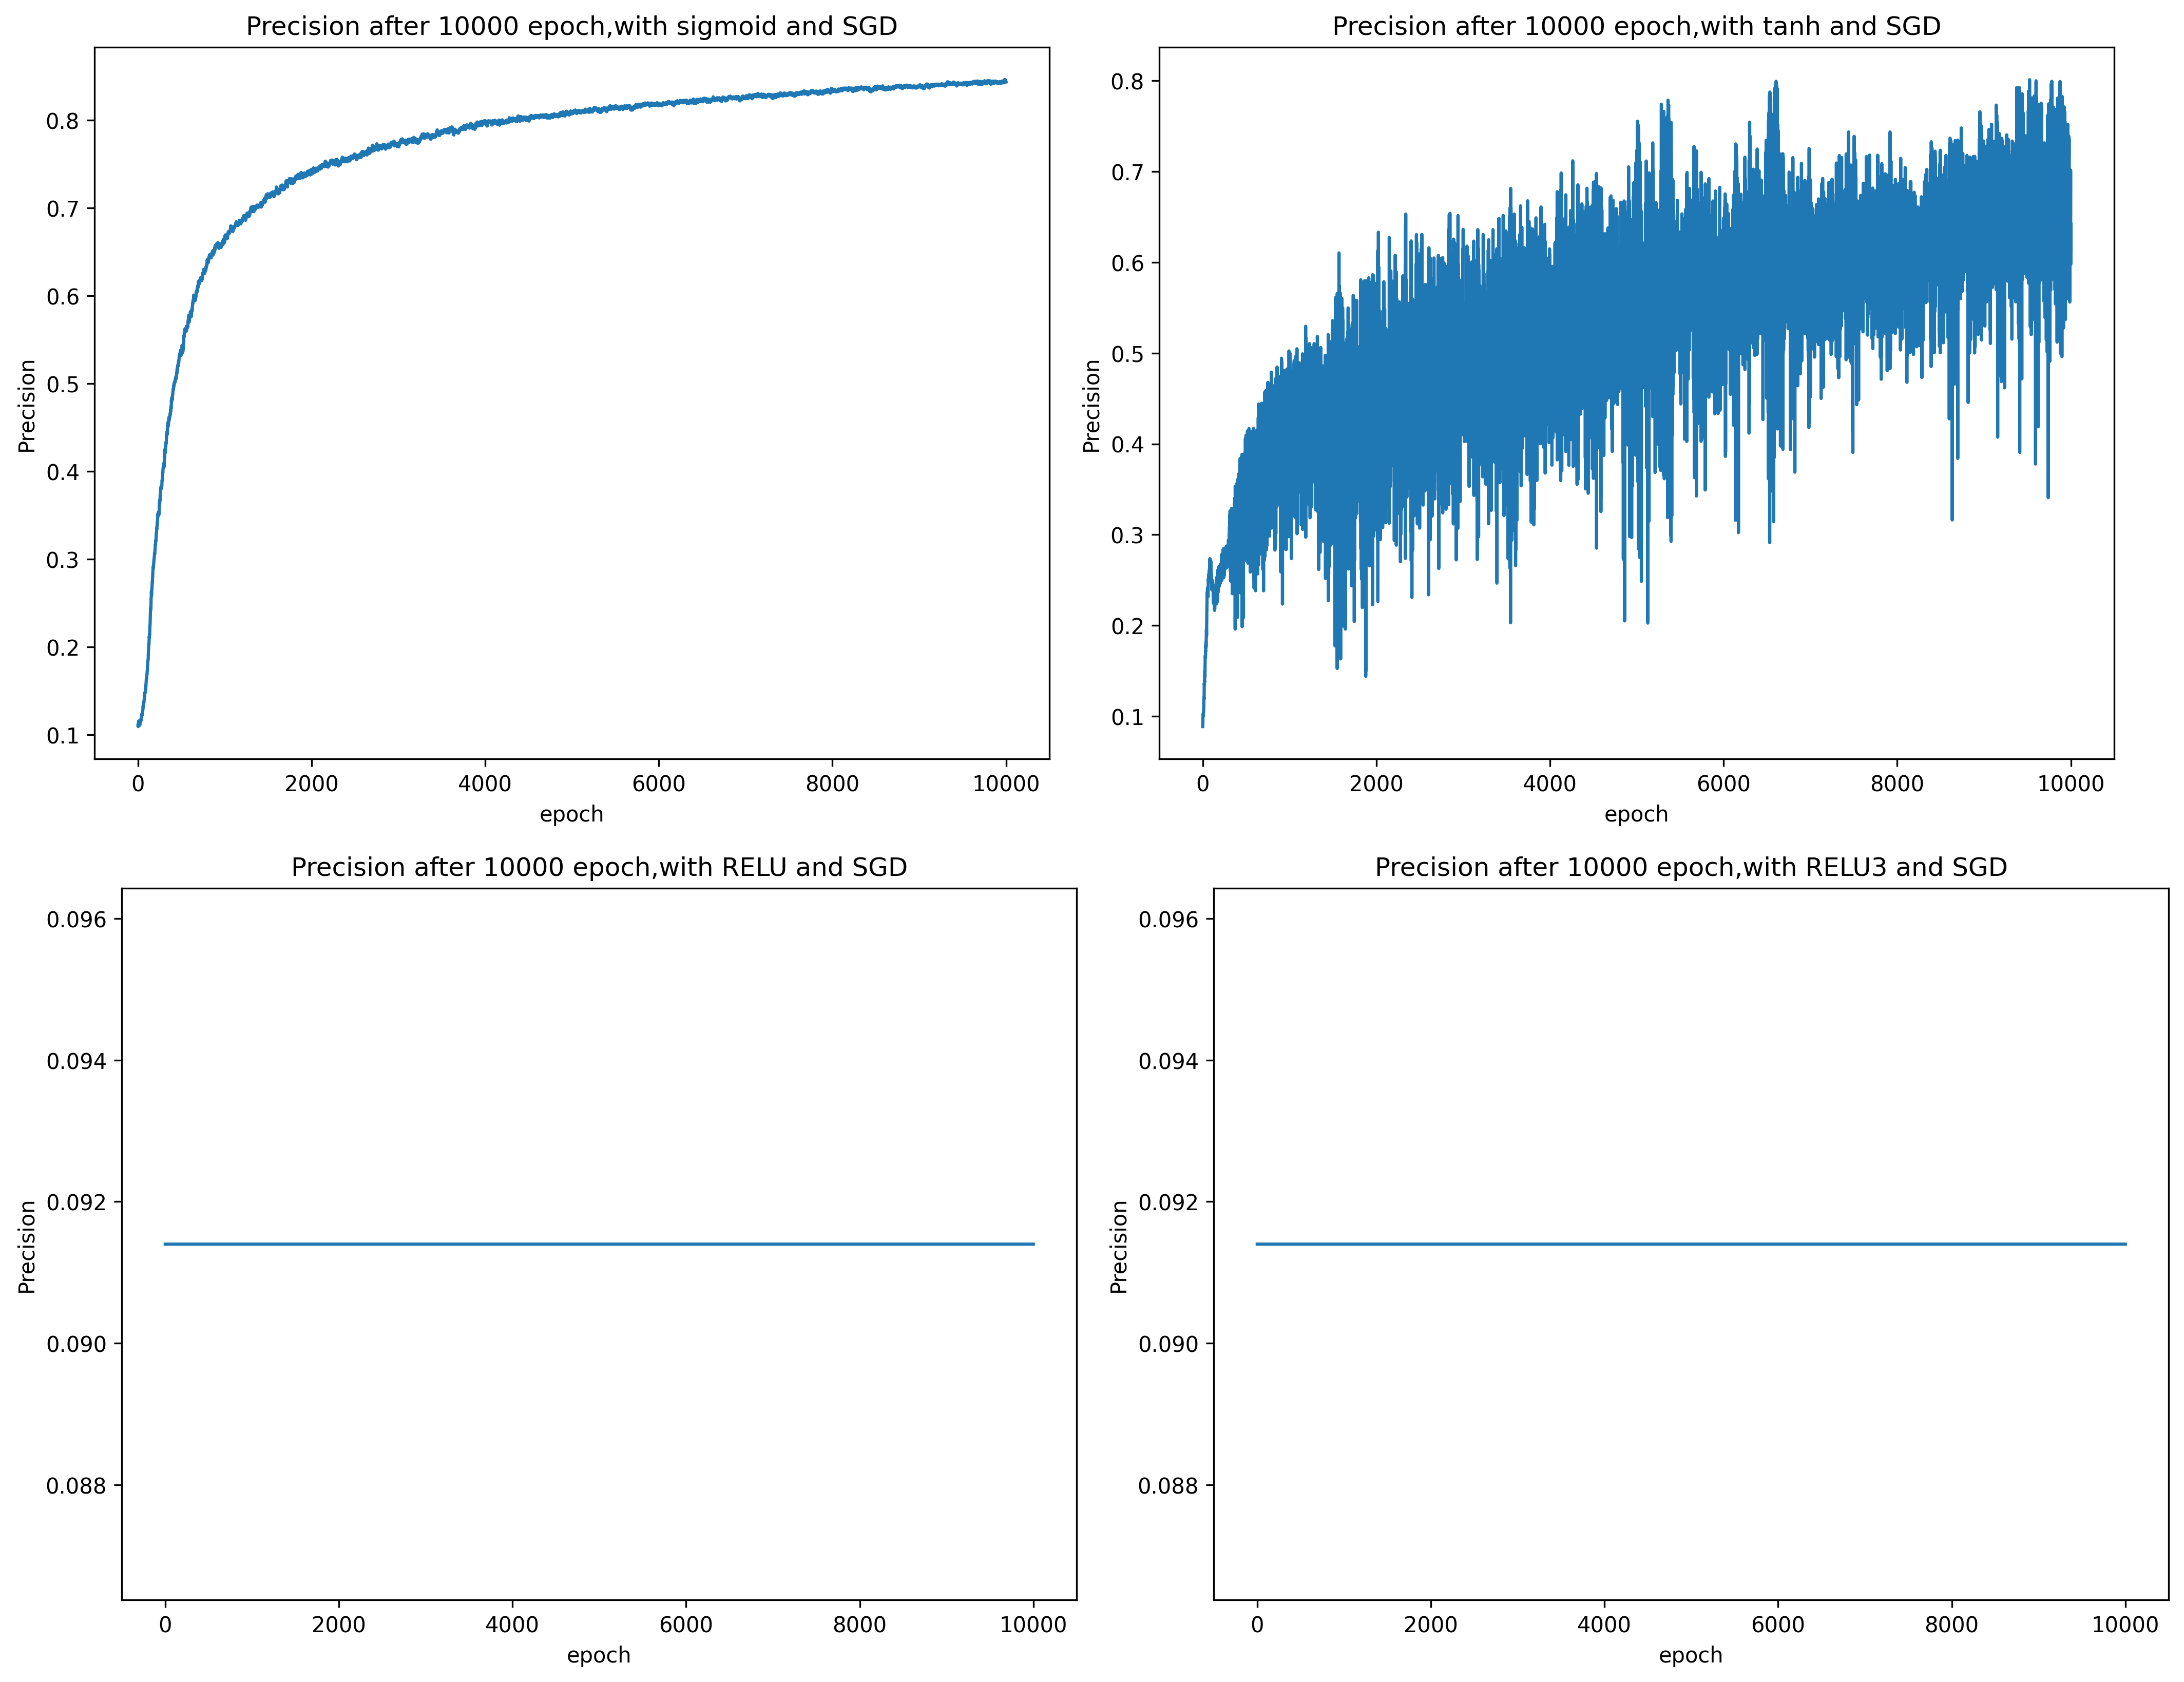
\includegraphics[width=\columnwidth]{SGD_4.png}
\caption{不同激活函数在 SGD 下的训练过程}
\end{figure}

\textbf{(2) Sigmoid + GD}

\begin{table}[H]
\centering
\scriptsize
\caption{Sigmoid + GD 结果}
\resizebox{\columnwidth}{!}{
\begin{tabular}{cccccc}
\toprule
训练轮次 & 学习率 & 训练样本数 & 测试样本数 & 训练集准确率 & 测试集准确率 \\
\midrule
10000 & 0.1 & 500 & 100 & 0.956 & 0.79 \\
\bottomrule
\end{tabular}}
\end{table}

\begin{figure}[H]
\centering
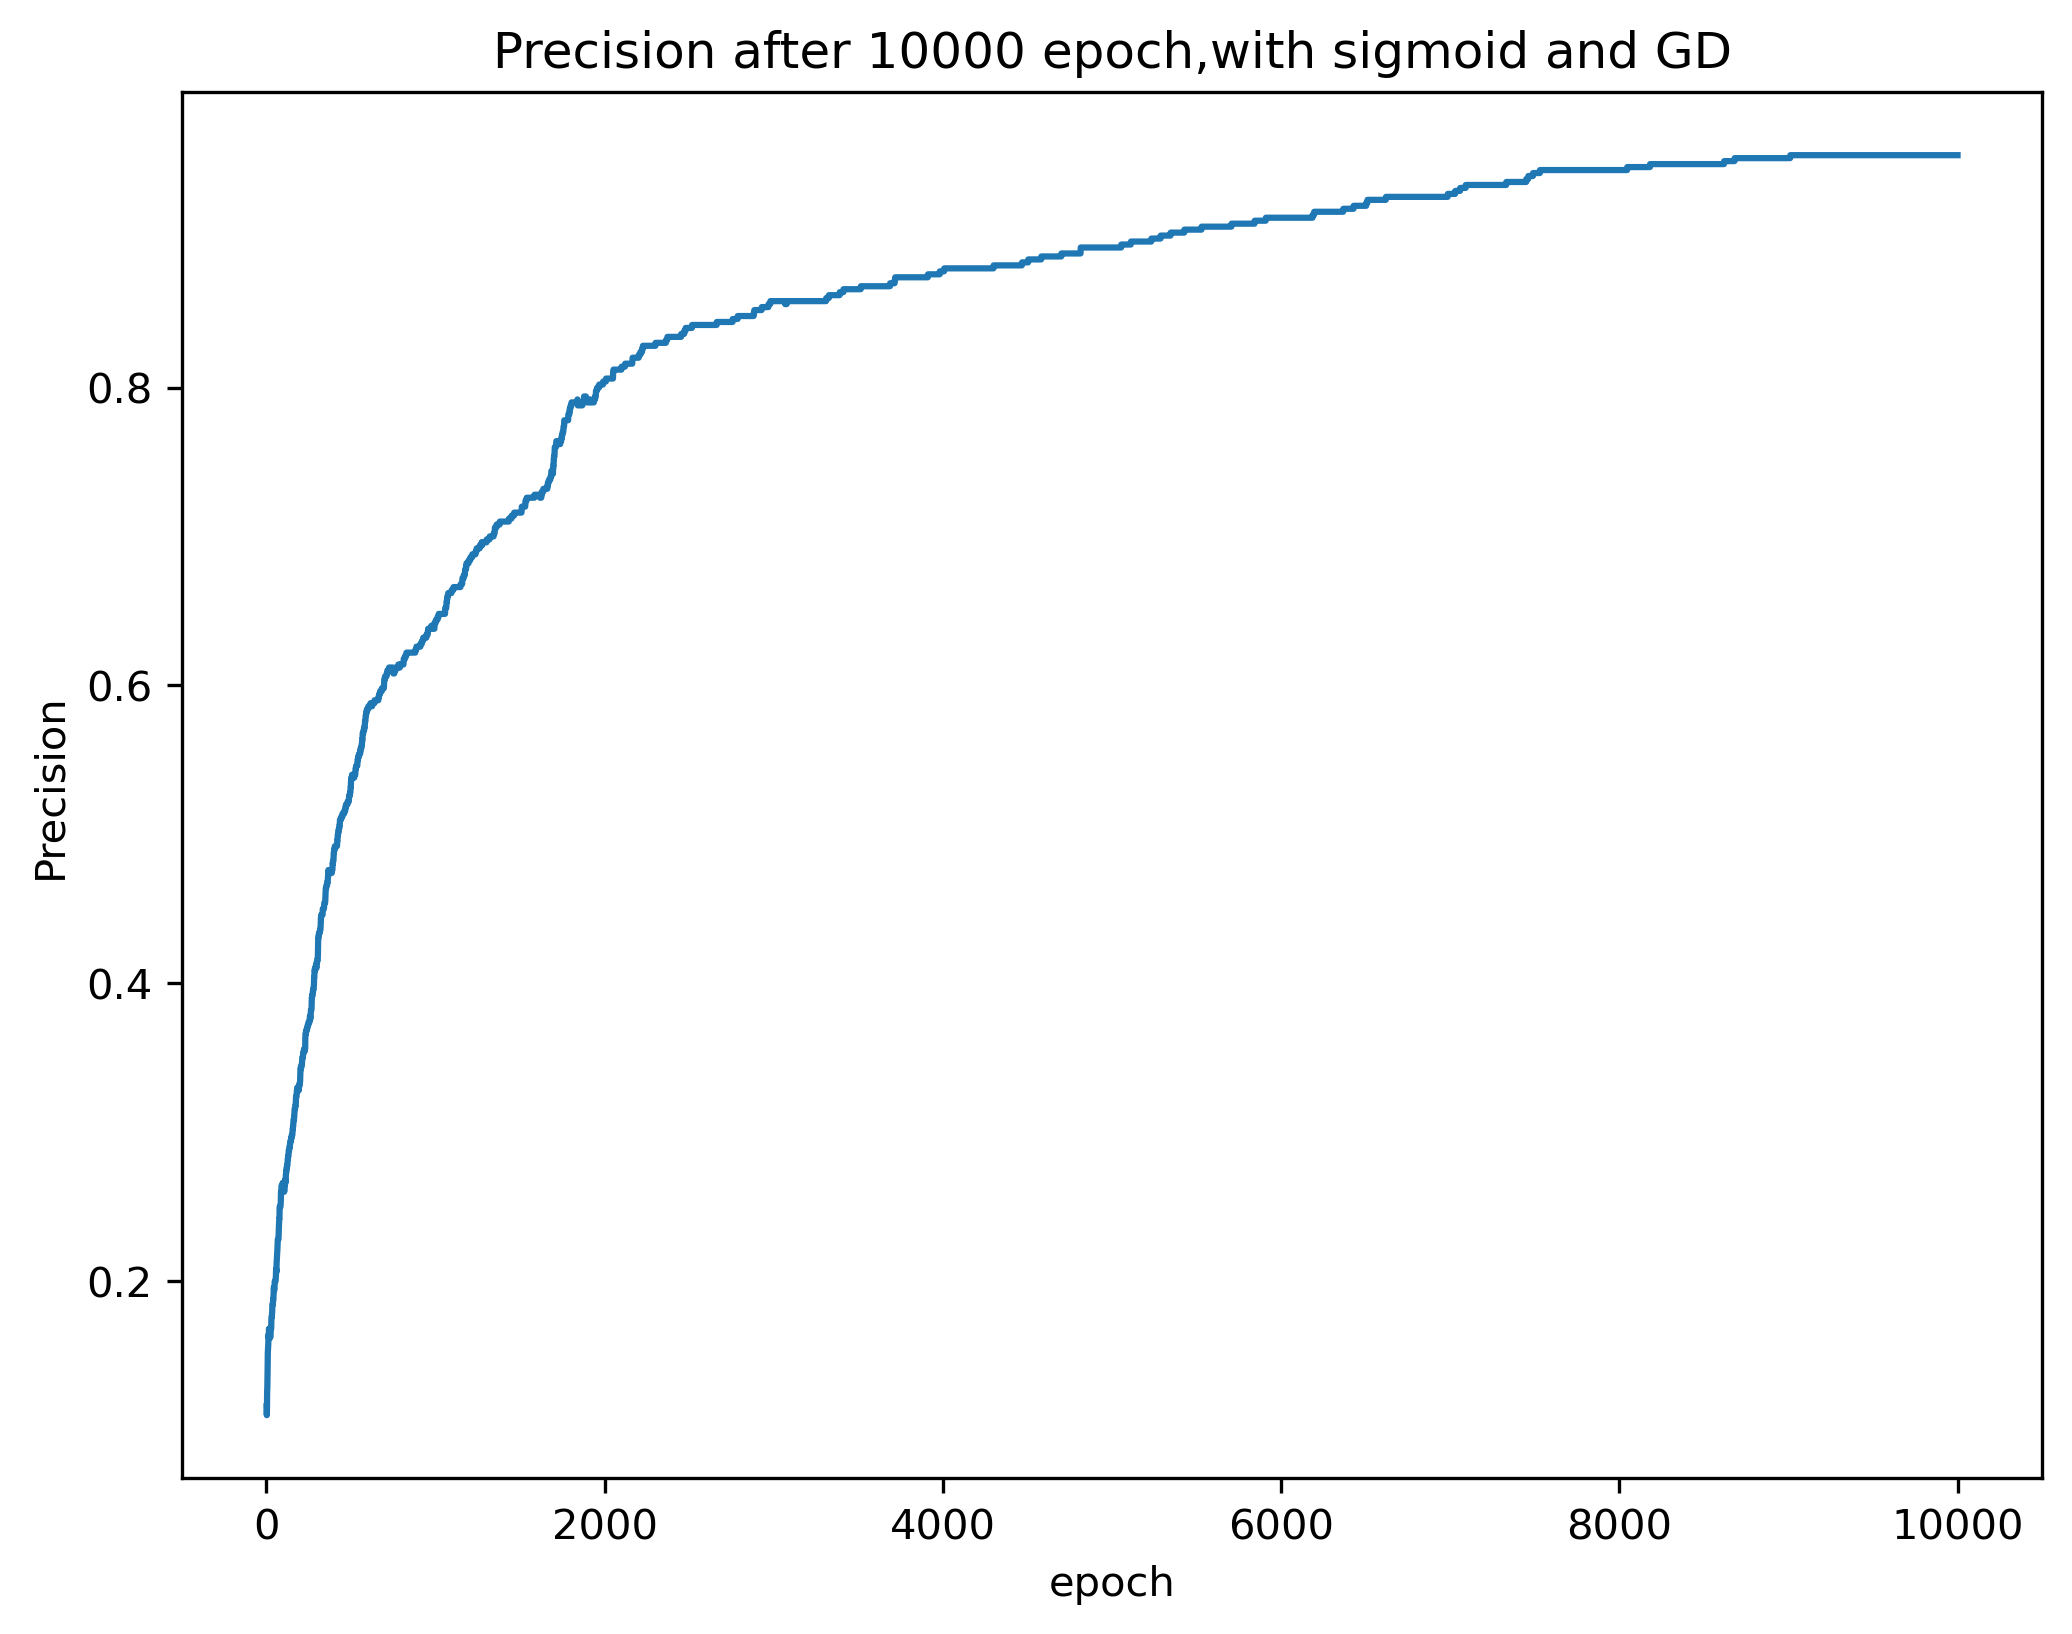
\includegraphics[width=\columnwidth]{sigmoid_GD.png}
\caption{Sigmoid + GD 训练曲线}
\end{figure}

\textbf{(3) Sigmoid + ADAM（学习率对比）}

\begin{table}[H]
\centering
\scriptsize
\caption{Sigmoid + ADAM 在不同学习率下的结果}
\resizebox{\columnwidth}{!}{
\begin{tabular}{cccccc}
\toprule
训练轮次 & 学习率 & 训练样本数 & 测试样本数 & 训练集准确率 & 测试集准确率 \\
\midrule
10000 & 0.1   & 5000 & 1000 & 0.1112 & 0.105 \\
10000 & 0.01  & 5000 & 1000 & 0.9896 & 0.835 \\
10000 & 0.001 & 5000 & 1000 & 0.9178 & 0.839 \\
\bottomrule
\end{tabular}}
\end{table}

\begin{figure}[H]
\centering
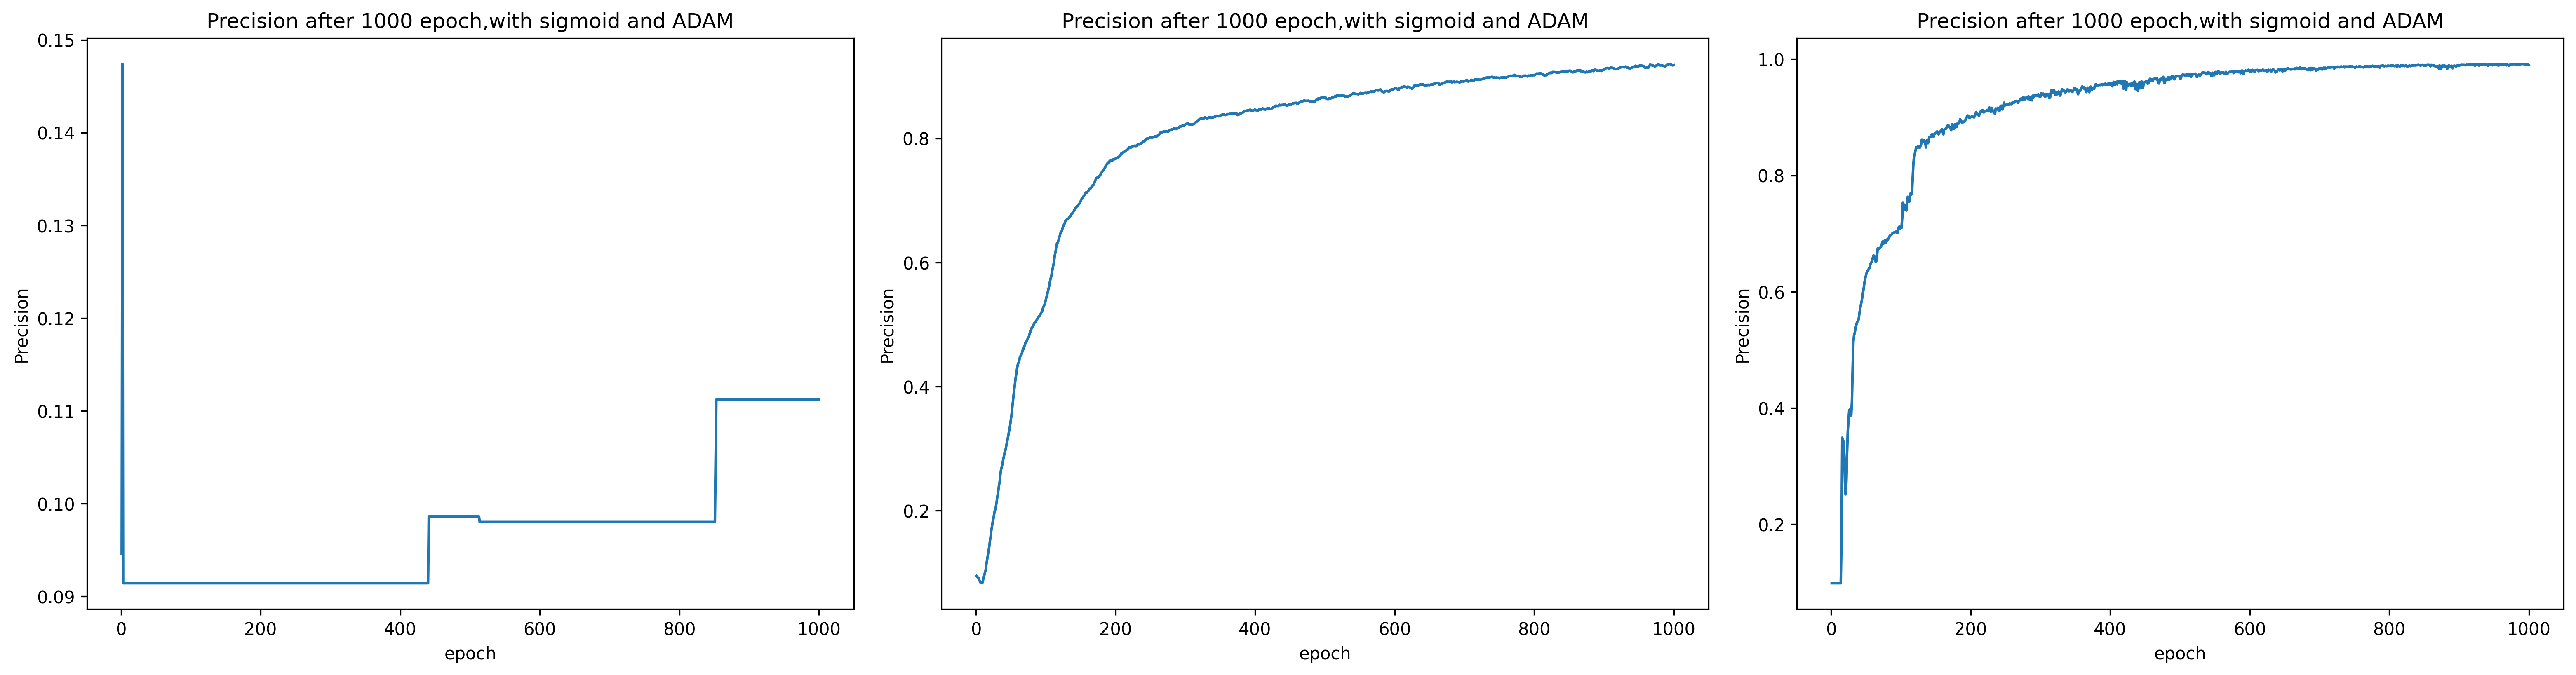
\includegraphics[width=\columnwidth]{sigmoid_ADAM.png}
\caption{ADAM 对比实验过程图}
\end{figure}

\begin{table}[H]
\centering
\scriptsize
\caption{主要结果汇总}
\resizebox{\columnwidth}{!}{
\begin{tabular}{cccc}
\toprule
实验组合 & 关键参数 & 测试准确率 & 结论 \\
\midrule
Sigmoid + SGD & lr=0.1 & 0.812 & 收敛稳定，表现较好 \\
Tanh + SGD & lr=0.1 & 0.535 & 训练波动较大 \\
ReLU/ReLU3 + SGD & lr=0.1 & 0.107 & 近似随机猜测 \\
Sigmoid + GD & 小样本(500/100) & 0.790 & 存在过拟合倾向 \\
Sigmoid + ADAM & lr=0.001\textasciitilde0.01 & 0.839 & 综合最优 \\
\bottomrule
\end{tabular}}
\end{table}

\subsection{结果分析}

从这组实验结果看，激活函数和优化器的搭配确实会直接影响模型效果。在同样使用 SGD、学习率都设为 0.1 的情况下，Sigmoid 可以做到 0.812，Tanh 只有 0.535，而 ReLU/ReLU3 基本停在 0.1 左右，几乎就是随机猜。这个结果说明在我当前这套初始化和参数设置下，ReLU 系列没有被很好地训练起来。
这一现象可能和当前实验设置有关：一方面，学习率 0.1 对 ReLU 来说可能偏大，早期更新不稳定；另一方面，若初始化方式与 ReLU 不匹配（如未使用 He 初始化），也可能使部分神经元较早进入“死亡 ReLU”状态，导致梯度传播受阻。

另外一个比较明显的现象是：Sigmoid + GD 的训练集准确率很高（0.956），但测试集只有 0.790。结合这组实验的样本量（500/100）来看，过拟合是比较合理的解释。ADAM 的对比也很典型：学习率 0.1 时几乎没法训练（0.105），降到 0.01 和 0.001 后马上提升到 0.835/0.839。也就是说，ADAM 不是“天然就好用”，学习率选得不合适一样会失败。

\subsection{结论}

\begin{enumerate}
\item 用手写 MLP 做 FashionMNIST 是可行的，参数设置合理时测试准确率可以稳定在 0.8 以上。
\item 这次实验里 Sigmoid 的表现最稳，Tanh 次之，ReLU/ReLU3 在当前设置下效果不理想。
\item 学习率非常关键，尤其在 ADAM 上体现得很明显；0.1 基本不可用，0.01 和 0.001 效果明显更好。
\item 如果按这份实验结果选一个默认方案，我会优先用 \textbf{Sigmoid + ADAM（学习率 0.001\textasciitilde0.01）}。
\end{enumerate}

\subsection{程序性能改进尝试}

\begin{itemize}
\item \textbf{从只跑 CPU 到支持 GPU}：最初版本全部是 NumPy，当前版本加了 CuPy 和 \texttt{use\_gpu}，有 GPU 时训练速度会快很多。
\item \textbf{统一计算接口}：用 \texttt{xp} 把 NumPy/CuPy 统一起来，前向、反向和评估都走同一套逻辑，代码更好维护，也少了很多重复判断。
\item \textbf{数值与数据处理更稳}：输入改成 \texttt{float32} 并做了归一化（除以 255），内存占用更小，训练过程也更稳定。
\item \textbf{设备转换更顺手}：增加了 \texttt{to\_gpu}、\texttt{to\_cpu}、\texttt{get\_xp} 这些函数，减少了手工搬运数据时容易犯错的地方。
\item \textbf{训练过程更可观察}：现在会记录 \texttt{precision\_history}/\texttt{perf\_history}，还能直接画曲线，这对调参很有帮助，不用只看最后一个准确率。
\end{itemize}

\section{代码附录}

以下代码片段来自 \texttt{demo\_mnist\_ann.py}，用于说明关键实现逻辑。

\textbf{1. 网络初始化与优化器选择}
\begin{lstlisting}
class NeuralNetwork:
    def __init__(self, layers, activation, opt_alg, use_gpu=True):
        self.use_gpu = use_gpu and GPU_AVAILABLE
        self.xp = cp if self.use_gpu else np

        if activation == 'sigmoid':
            self.activation = sigmoid
            self.activation_deriv = sigmoid_deriv
        elif activation == 'tanh':
            self.activation = tanh
            self.activation_deriv = tanh_deriv

        if opt_alg == 'GD':
            self.opt = self.GD
        elif opt_alg == 'SGD':
            self.opt = self.SGD
        elif opt_alg == 'ADAM':
            self.opt = self.ADAM
\end{lstlisting}

\textbf{2. 反向传播梯度计算}
\begin{lstlisting}
xp = self.xp
for i in range(n_w-1, -1, -1):
    if i == n_w-1:
        delta[i] = error * self.activation_deriv(z[i])
    else:
        delta[i] = xp.dot(self.weights[i+1].T, delta[i+1]) * \
                   self.activation_deriv(z[i])

for i in range(n_w):
    dweights.append(xp.dot(delta[i], K[i].T))
    dthetas.append(delta[i])
\end{lstlisting}

\textbf{3. 训练与测试流程}
\begin{lstlisting}
layers = np.array([X.shape[0], 128, 64, Y.shape[0]])
Net = NeuralNetwork(layers, 'sigmoid', 'GD', use_gpu=True)
Net.train(X, Y, 1, 0.1,10000)
Net.plot_precision("sigmoid_GD.png")

testX_dev = to_gpu(testX) if GPU_AVAILABLE else testX
testY_dev = to_gpu(testY) if GPU_AVAILABLE else testY
output = Net.propagation(testX_dev, 1)
xp = cp if GPU_AVAILABLE else np
true = int(to_cpu(xp.sum(xp.argmax(testY_dev, axis=0)
          == xp.argmax(output, axis=0))))
print("test precision:", true / testX.shape[1])
\end{lstlisting}

\end{document}
